\scanpage{84}
% archive foliation: 83
\uline{Calculs} pour $T_\ell(\mathbf G_m)\inserted{{}=\mathbf Q_\ell(1)}$ et $\mathbf G_m$.

$X$ de type fini sur $\mathbf Z$

\[
H^0(X,\mathbf Q_\ell(1))\deleted{\unsure{\mathbf G_m}}=0
\]
\figure{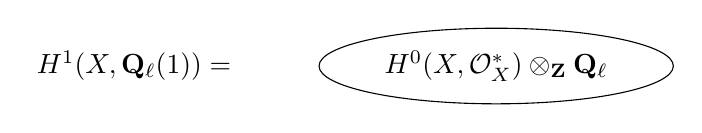
\begin{tikzpicture}
\node at (0,0) {$H^1(X,\mathbf Q_\ell(1))=$};
\node at (4.6,0) {$H^0(X,\mathcal O_X^*)\otimes_{\mathbf Z}\mathbf Q_\ell$};
\draw (4.6,0) ellipse (2.25 and .48);
\end{tikzpicture}}
\figure{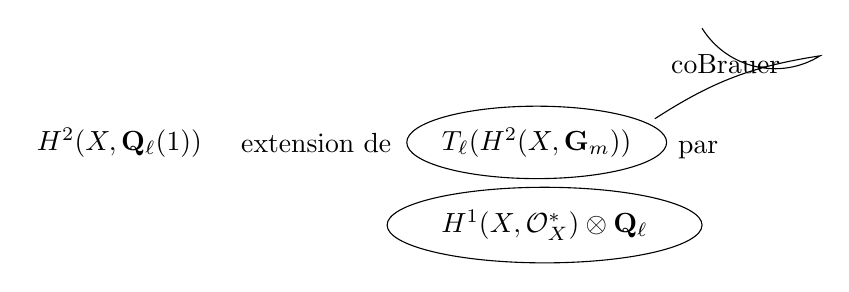
\begin{tikzpicture}
\node at (0,0) {$H^2(X,\mathbf Q_\ell(1))$};
\node at (2.5,0) {extension de};
\node at (5.3,0) {$T_\ell(H^2(X,\mathbf G_m))$};
\draw (5.3,0) ellipse (1.65 and .46);
\node at (7.35,-.1) {par};
\node at (5.4,-1.05) {$H^1(X,\mathcal O_X^*)\otimes\mathbf Q_\ell$};
\draw (5.4,-1.05) ellipse (2 and .48);
\node at (7.7,1) {\uline{coBrauer}};
\draw (6.8,.3) to[bend left=12] (8.9,1.1) to[bend left=45] (7.4,1.45);
\end{tikzpicture}}
\[
H^3(X,\mathbf Q_\ell(1))\simeq T_\ell(H^3(X,\mathbf G_m))\quad\text{est ce qu'il peut}
\]
\hfill [p.ex. $\mathbf Z_\ell$ si $X$ \deleted{\unsure{modèle}} \unsure{cour.} d'un
corps de fonctions d'une variable sur $\mathbf F_p$]

\[
\begin{array}{c}
H^i(X,\mathbf Q_\ell(1))=0\\
\Vert\\
T_\ell(H^i(X,\mathbf G_m))
\end{array}
\qquad\text{si }i\ge4\qquad ??
\]

On conjecture (C. Artin) que $H^2(X,\mathbf G_m)=$ groupe
fini si $X$ propre sur $\mathbf Z$. \deleted{Alors si}\inserted{Vrai}
si $X$ courbe projective lisse sur $\mathbf F_p$, mais
faux quand on lui enlève des pts --- le
rang du $H^{\unsure{2|3}}$ augmente d'autant.

$H^{\unsure{3|2}}(X,\mathbf Q_\ell(1))$ : quelle est sa taille [il décroît en
passant à un ouvert de $X$]
